\documentclass{beamer}

\mode<presentation>
{
  \usetheme{Darmstadt}      % or try Darmstadt, Madrid, Warsaw, ...
  \usecolortheme{default} % or try albatross, beaver, crane, ...
  \usefonttheme{serif}  % or try serif, structurebold, ...
  \setbeamertemplate{navigation symbols}{}
  \setbeamertemplate{caption}[numbered]
} 
 
\usepackage[utf8]{inputenc}
\usepackage[]{algorithm2e}

%Information to be included in the title page:
\title{Nat-Sci II Presentation: \\
Editing of Pig DNA May Lead to More Organs for People}
\author{YD Choi, Amy Jung, Vaughn Tajirian, Katie Westerlund }
\institute{New York University}
 
\begin{document}
 
\frame{\titlepage} 

\begin{frame}
\frametitle{The Article under Investigation}
\begin{itemize} 
\item ``Editing of Pig DNA May Lead to More Organs for People," appeared in
New York times Science section (10/15/15). Written by Carl Zimmer.
\end{itemize}
\begin{figure}[h!]
  \centering
    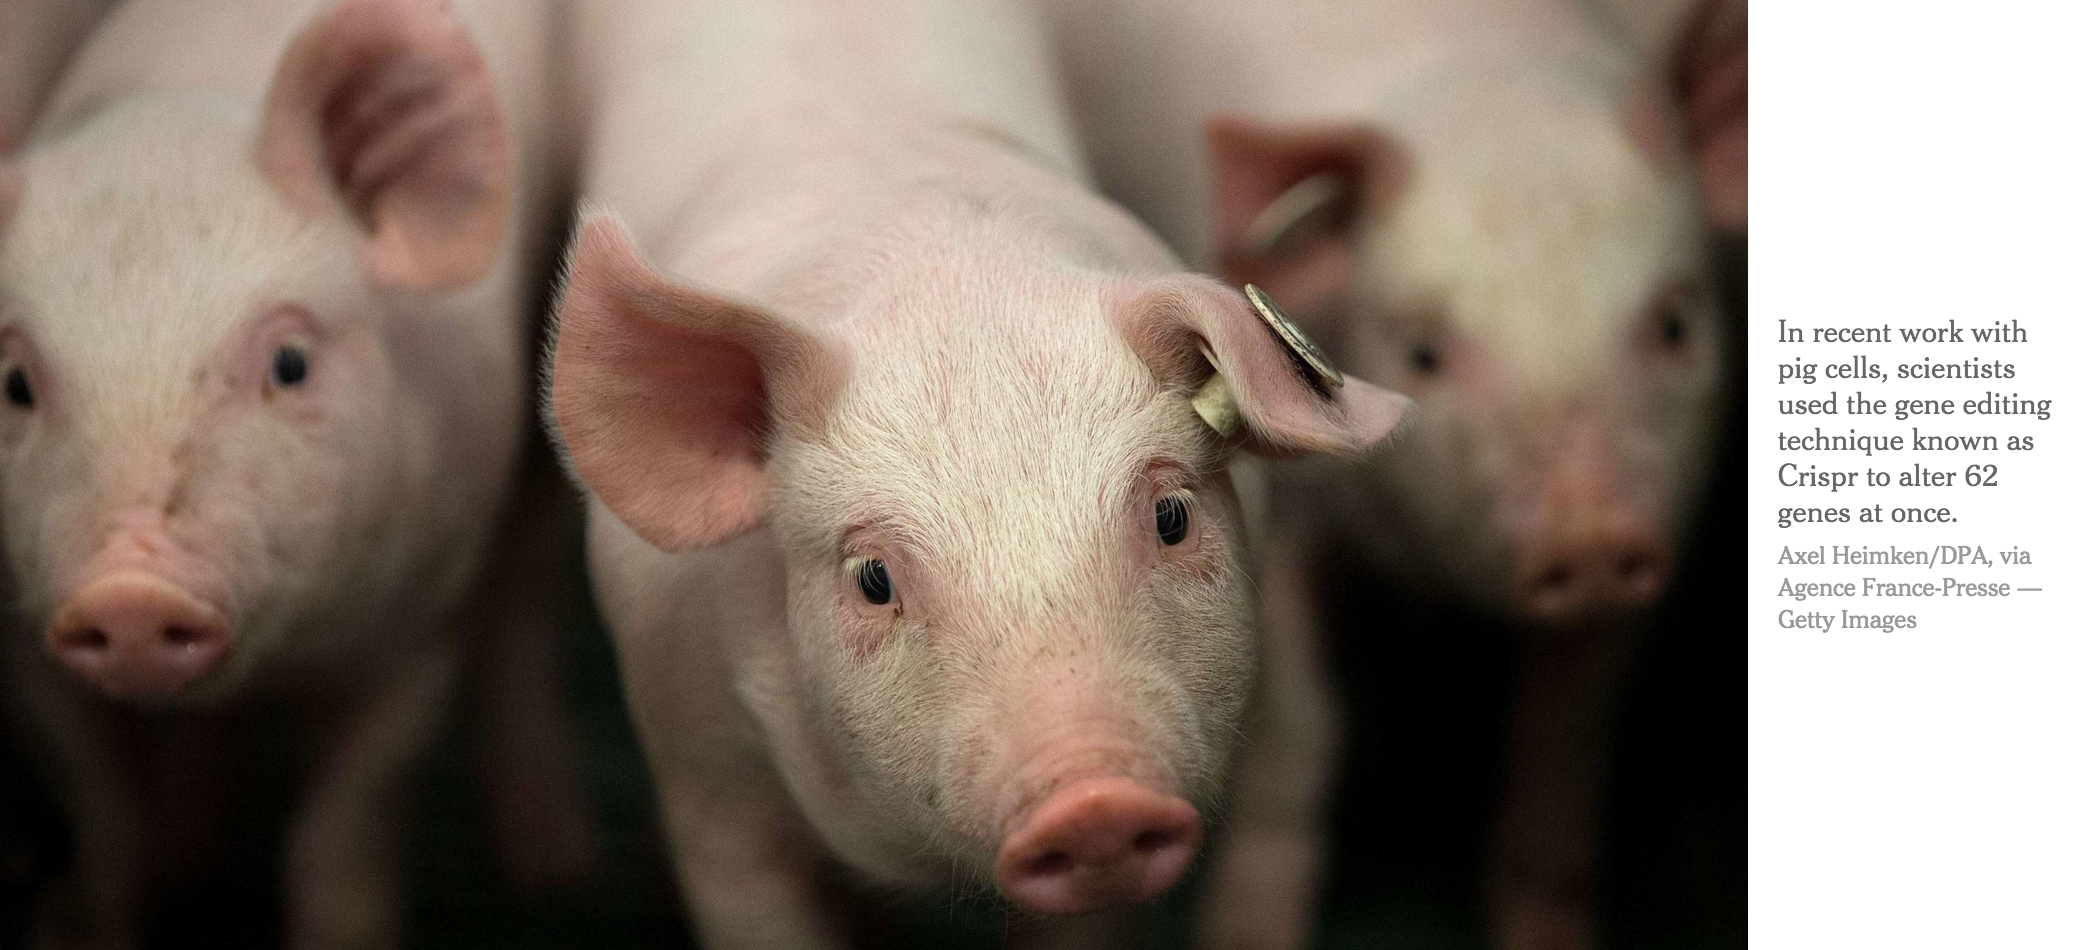
\includegraphics[width=1\textwidth]{edit-pigs.png}
\end{figure}
\end{frame}

\begin{frame}
\frametitle{Genetics meets Surgical Technologies: \\
CRISPR and Xenotransplantation}
\begin{itemize}
\item CRISPR : A recently developed method for 
``editing genes."
\item Xenotransplantation :
The transplantation of living cells, tissues or organs
from one species to another. 
\item It has been recently shown that a particular
complication that arises in
xenotransplantation, using pig organs,
can be solved through gene-editing via CRISPR. 
\end{itemize}
\end{frame}

\begin{frame}
\frametitle{Development from Genetics: CRISPR}
\begin{itemize}
\item In October of 2015, scientists gathered at the National Academy of Sciences
in Washington to talk about CRISPR, a new method for editing genes.

\item Carl Zimmer claims that ``In the past couple of years, 
the technique has become so powerful and accessible that many experts are 
calling for limits on its potential uses — especially altering human 
embryos with changes that could be inherited by future generations."
\end{itemize}
\end{frame}

\begin{frame}
\frametitle{CRISPR: a new method for editing genes I}
\begin{itemize}
\item
In the CRISPR, the new spacer spacer sequences match part of the infecting phage genome’s sequence.
\item In CRISPR's protecting the body, they interfere with a phage infection
\end{itemize}
\begin{figure}[h!]
  \centering
    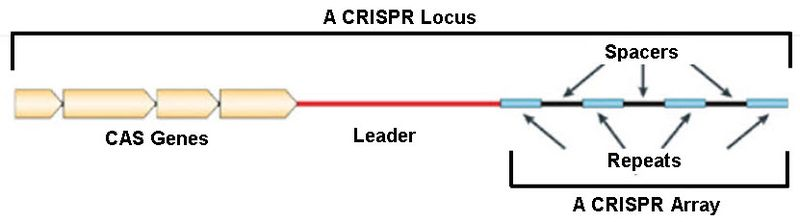
\includegraphics[width=1\textwidth]{crispr.jpg}
\end{figure}
\end{frame}


\begin{frame}
\frametitle{CRISPR: a new method for editing genes II}
\begin{itemize}
\item  Recent discoveries tell us that CRISPR defense does not block phage absorbtion.
\item Does not involve a restriction-modification system (bacteria’s way to protect themselves from foreign DNA).
\item And is not an abortive infection mechanism (blocks phage multiplication, resulting in premature death for the bacteria).
\end{itemize}
\end{frame}

\begin{frame}
\frametitle{CRISPR: a new method for editing genes III}
\begin{itemize}
\item The CRISPR is transcribed as a single, very long strand of RNA.
\item The strand of RNA is cut at a certain ``
site in each to repeat and yield the mature CRISPR RNAs (crRNAs).”
\item Every crRNA contains one entire spacer sequence plus recognizable "handles." 
\item  The now single spacers (after crRNA is cut) are processed into active defense agents and are continuously on guard for their matching phages and 
plasmids.

\end{itemize}
\end{frame}

\begin{frame}
\frametitle{Complications of Xenotransplantation \\with Pig Organs I}
\begin{itemize}
\item
In the 1990s, xenotransplantation, a technique that uses pig organs in humans, has been topic much discussed by scientists. They have hoped that the organs from the pigs could be cleaned from the harmful viruses and pathogens that would enter the human host and ultimately harm them. 
\end{itemize}
\begin{figure}[h!]
  \centering
    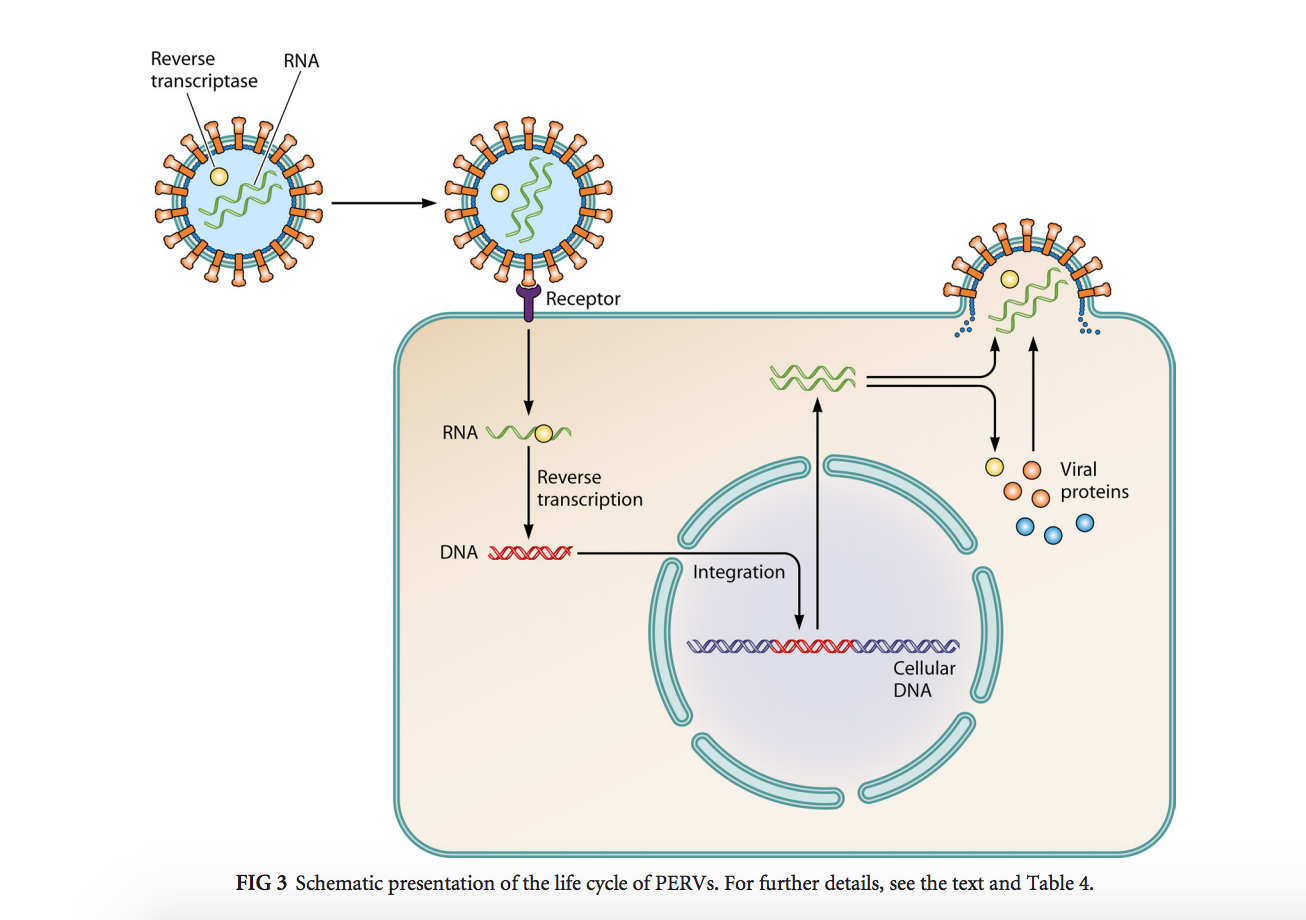
\includegraphics[width=0.5\textwidth]{lifecycle.png}
\end{figure}
\end{frame}

\begin{frame}
\frametitle{Complications of Xenotransplantation \\ with Pig Organs II}
\begin{itemize}
\item
However, the issues with this is that in the pig’s DNA there are viral genes. These genes are called endogenous retroviruses; which humans also have. 
\item
The one found in pigs (PERVs) can produce viruses that infect other pig cells. Unfortunately, when mixed with human cells, they are also infected. 
\end{itemize}
\end{frame}


\begin{frame}
\frametitle{Gene-editing Solution to the Complications}
\begin{itemize}
\item
This road block seamed impossible to get rid off to scientists because they were part of the pig’s genome. 
\item
However, Dr. Church was able to figure out a method to disable the PERVs. They started off by finding out there are 62 PERVs found in each cell, and that the PERVs had almost identical DNA. 
\item
What Dr. Church did was design a new set of genes and place them into the pig cells. These new genes created enzymes would find the PERVs and cut them out from the DNA. Within two weeks, the pig cells had changed all the viral DNA. 
\item
Dr. Church was able to accomplish this by creating only one molecule, not 62, to alter the 62 genes.
\end{itemize}
\end{frame}

\begin{frame}
\frametitle{Conclusion}
\begin{itemize}
\item This new discovery in modifying pig genes has opened many new doors in the possibilities organ transplant.
\item It finally gives scientist the chance to create new sustainable organs that can be safely used in humans. 
\item
CRISPR is great not only for modifying pig genes, but also for allowing scientist to modify a wide-range of animal and even human genes. 
\end{itemize} 
\end{frame}


\end{document}
